\documentclass[11pt]{article}

\usepackage[utf8]{inputenc}
\usepackage[T1]{fontenc}
\usepackage{amsmath,amssymb}
\usepackage{booktabs}
\usepackage{graphicx}
\usepackage{algorithm}
\usepackage{algpseudocode}
\usepackage[numbers,sort&compress]{natbib}
\usepackage{hyperref}
\usepackage{xcolor}
\usepackage{geometry}
\geometry{margin=1in}
\hypersetup{colorlinks=true,linkcolor=blue!50!black,citecolor=blue!50!black,urlcolor=blue!50!black}

\newcommand{\R}{\mathbb{R}}
\newcommand{\Fforce}{F}
\newcommand{\NWM}{\textsc{NWM}}

\title{\NWM: Negative Weight Mapping\\
\large A Non-Parametric Potential-Field Framework for Reinforcement Learning}

\author{CastermustOfficial\\
\texttt{https://github.com/CastermustOfficial/NWM}}

\date{\today}

\begin{document}
\maketitle

\begin{abstract}
We present \emph{Negative Weight Mapping} (\NWM), a non-parametric reinforcement
learning framework that represents an agent's experience as a persistent
\emph{potential field} over the observation space. Rather than training a value
network or a policy by gradient descent, \NWM{} accumulates a compact set of
\emph{centroids}---prototypical states that store per-action success and failure
statistics---and selects actions by aggregating attractive (success) and
repulsive (failure) forces from nearby centroids. Two mechanisms give the memory
long-term stability: a \emph{Dynamic Smart Lock} that protects high-confidence
prototypes from being overwritten, and a \emph{Fear \& Greed} decision rule that
rejects dangerous actions before maximizing reward. To act well under sparse
reward, \NWM{} additionally uses \emph{temporally-correlated (sticky)
exploration}, which repeats exploratory actions to build the sustained momentum
that uniform noise cannot---and whose repeat probability can self-tune from the
agent's own reward history. A further mechanism propagates value backwards along
a graph of observed centroid transitions, letting outcomes stitch across
episodes without disturbing the absolute score scale the decision rule depends
on. We formalize the method and evaluate it against three baselines---a uniform
random policy, tabular Q-learning with state aggregation, and a Deep Q-Network
(DQN)---on three classic-control benchmarks spanning a difficulty gradient
(CartPole, Acrobot, MountainCar), using one configuration shared across all
tasks, $20$ seeds, and paired per-seed significance tests. \NWM{} decisively
solves the sparse-reward MountainCar task, where every baseline including DQN
fails to reach the goal even once ($+64.7$ return, $p<10^{-3}$); it is
competitive with DQN on dense CartPole, though the gap in its favour is not
statistically established; and it trails DQN on the longer-horizon Acrobot. The
MountainCar result reframes a failure mode often attributed to non-bootstrapping
methods: there the obstacle is \emph{exploration}, not temporal credit
assignment, and a single task-agnostic change removes it. We also report a
methodological finding that applies beyond this system. Earlier versions of this
study used five seeds, a sample size at which the across-seed standard deviation
of these benchmarks ($130$--$140$ return units) makes differences below roughly
$120$ units indistinguishable from noise; several conclusions we had drawn on
that basis---including a mechanism trade-off we had shipped and documented---do
not survive at $20$ seeds. We report the corrected comparisons, including one in
which fixing a bootstrapping bug in our own baselines reverses a result in
DQN's favour. All code, seeds, and figures are released to make the study fully
reproducible.
\end{abstract}

\section{Introduction}
\label{sec:intro}

Most modern reinforcement learning (RL) methods are \emph{parametric}: a neural
network compresses experience into weights updated by gradient descent
\citep{mnih2015human,schulman2017proximal}. Parametric value learning is
powerful but has well-known costs: it is sample-hungry, sensitive to
hyperparameters, prone to catastrophic forgetting, and notoriously difficult to
reproduce \citep{henderson2018deep}. A complementary line of work is
\emph{non-parametric} or \emph{episodic} control, which stores experience
explicitly and acts by similarity to past situations
\citep{blundell2016model,pritzel2017neural}. Such methods can learn quickly from
few interactions because a single informative experience is immediately usable,
without waiting for it to be amortized into network weights.

\NWM{} sits in this non-parametric family but takes an unusual inspiration: the
\emph{artificial potential field}, a classic idea from robot motion planning in
which goals exert attractive forces and obstacles exert repulsive ones
\citep{khatib1986real}. \NWM{} treats past \emph{successes} as attractors and
past \emph{failures} as repulsors in the observation space, so that action
selection reduces to following the net force at the current state. The name
\emph{Negative Weight Mapping} refers to the explicit modelling of negative
(repulsive) experience, which is used not merely to lower a value estimate but
to actively veto risky actions.

This paper makes the original repository's method precise and subjects it to a
controlled empirical study. Concretely, we contribute:
\begin{enumerate}
  \item A formal description of the \NWM{} memory, force model, and decision rule
  (Section~\ref{sec:method}), including the Dynamic Smart Lock and Fear \& Greed
  mechanisms that were previously only described informally, and a
  temporally-correlated (sticky) exploration rule for sparse-reward tasks.
  \item A reproducible benchmark harness comparing \NWM{} against Random,
  tabular Q-learning, and DQN across three environments and $20$ seeds, with a
  fixed greedy-evaluation protocol and aggregate statistics
  (Section~\ref{sec:experiments}).
  \item An analysis of the results (Section~\ref{sec:results}) that identifies
  the regimes in which a potential-field method is competitive, together with an
  explicit discussion of its limitations (Section~\ref{sec:limitations}).
  \item A methodological correction to our own earlier reporting
  (Section~\ref{par:power}): at the five-seed sample size these benchmarks are
  routinely run with, the across-seed noise exceeds most of the effects being
  claimed. We show a mechanism ablation reversing sign between two five-seed
  samples, retract the conclusions we had drawn that way---including a
  trade-off we had shipped as a default---and re-report everything at $20$
  seeds with paired tests.
\end{enumerate}

\section{Related Work}
\label{sec:related}

\paragraph{Value-based RL.} Q-learning \citep{watkins1992q} learns an
action-value function by temporal-difference updates; with function
approximation and experience replay it scales to high-dimensional inputs as DQN
\citep{mnih2015human,lin1992self}. We use both a tabular variant (with state
aggregation) and DQN as baselines.

\paragraph{Episodic and non-parametric control.} Model-Free Episodic Control
\citep{blundell2016model} and Neural Episodic Control \citep{pritzel2017neural}
store returns in a growing table keyed by (embedded) states and act by
$k$-nearest-neighbour lookup, achieving strong early sample efficiency. \NWM{}
shares the store-and-retrieve philosophy but differs in three ways: (i) it
aggregates experience into a bounded set of merged \emph{centroids} rather than
retaining individual transitions; (ii) it stores a \emph{signed force} per
action rather than a raw return estimate; and (iii) it separates
\emph{repulsion} into its own spatial-decay and veto pathway.

\paragraph{Potential fields.} Artificial potential fields
\citep{khatib1986real} are a staple of reactive control and motion planning.
\NWM{} imports the attractive/repulsive metaphor into RL by learning the field
from returns rather than from a hand-specified geometry.

\section{Method}
\label{sec:method}

\subsection{Setup and notation}
We consider a Markov decision process with observation space
$\mathcal{S}\subseteq\R^{d}$ and a finite action set
$\mathcal{A}=\{0,\dots,K{-}1\}$. Observations are $z$-score normalized online
using running mean and variance maintained with Welford's algorithm
\citep{welford1962note}; we write $\tilde{x}$ for the normalized observation.

\subsection{Persistent potential field}
The memory is a bounded collection of centroids
$\mathcal{M}=\{c_1,\dots,c_N\}$, $N\le N_{\max}$. Each centroid $c_i$ stores
\begin{itemize}
  \item a prototype location $\mu_i\in\R^{d}$ (a running mean of the normalized
  states merged into it) and a visit count $n_i$;
  \item per-action statistics $\{(s_{i,a}, n_{i,a}, q^{2}_{i,a})\}_{a}$
  accumulating the sum, count, and sum of squares of the scores observed for
  action $a$; and
  \item a boolean \emph{lock} flag $\ell_i$.
\end{itemize}
The average score of action $a$ at centroid $i$ is
$\bar q_{i,a}=s_{i,a}/n_{i,a}$.

\paragraph{Insertion and merging.} A new experience
$(\tilde x, a, \sigma)$ with score $\sigma\in[0,1]$ (defined below) is routed to
the nearest centroid $j=\arg\min_i \lVert \mu_i-\tilde x\rVert$. If
$\lVert \mu_j-\tilde x\rVert < \tau_{\mathrm{merge}}$ it is merged into $c_j$;
otherwise a new centroid is created. Merging uses an exponential moving average
with \emph{progressive stiffness}: the mixing rate is $\alpha=1/(n_j{+}1)$, and
$\alpha=1/(2n_j)$ once $n_j>50$, so that well-established prototypes drift
slowly. When $N$ exceeds capacity, unlocked centroids are pruned by a value
score $n_i\big((\bar q_i-0.5)^2+0.1\big)$ that favours frequently-visited,
strongly-signed prototypes; locked centroids are always retained.

\subsection{Score assignment}
Learning is episodic. At the end of an episode with return $G$, we compute a
\emph{percentile score} $p\in[0,1]$ equal to the rank of $G$ among all
historical returns, so that scores are self-calibrating across environments with
different reward scales. A temporal weight $w_t=0.4+0.6\,t/T$ emphasizes later
steps of a length-$T$ episode, and the score written for step $t$ is
$\sigma_t=\mathrm{clip}(p\,w_t,0,1)$.

\paragraph{Neutral-blended credit.} Scaling $p$ by $w_t$ drives the early steps
of a \emph{good} episode toward $0$---i.e.\ toward repulsion---even though those
steps were not at fault. We therefore blend toward the neutral score $0.5$
rather than toward $0$,
\begin{equation}
\sigma_t=\mathrm{clip}\!\left(0.5+(p-0.5)\,w_t,\;0,\;1\right),
\label{eq:creditblend}
\end{equation}
so that early steps of a good episode stay mildly attractive and early steps of
a bad one stay mildly repulsive. Equation~\eqref{eq:creditblend} is used
throughout the reported benchmark.

\paragraph{Truncation-aware credit.} The ramp $w_t$ implicitly assumes the end of
an episode explains its outcome, which is true for a true terminal event and
false for a time-limit truncation. Given the \texttt{terminated}/\texttt{truncated}
distinction we therefore set $w_t$ per episode type: a poor episode ending in a
genuine terminal event keeps the late-step ramp (the ending did cause the
failure); a poor \emph{truncated} episode---aimless until the clock ran
out---receives flat mild credit, since no particular step is to blame; and a good
truncated episode, which survived the entire limit, receives full flat credit
instead of under-crediting the early steps that kept it alive.

\paragraph{Sign-aware quality gate.} A \emph{dynamic quality gate} caps
$\sigma_t\le 0.6$ (preventing attraction, which needs $\bar q>0.6$, and locking,
which needs $\bar q>0.8$) for episodes that are not genuinely above trend. The
natural threshold $\max(40,\,1.25\,\bar G_{\text{recent}})$ is correct only for
positive returns: when $\bar G_{\text{recent}}<0$---as it is throughout training
on Acrobot and MountainCar---the term $1.25\,\bar G_{\text{recent}}$ is
\emph{smaller} than $\bar G_{\text{recent}}$ and the constant $40$ dominates,
capping every episode at $0.6$ and silently disabling both attraction and the
Dynamic Smart Lock on exactly the tasks that need them. We therefore make the
gate sign-aware, requiring an episode to beat its recent average by a fixed
\emph{relative} margin regardless of sign:
\begin{equation}
G \;\ge\; \bar G_{\text{recent}} + \tfrac{1}{4}\,\bigl|\bar G_{\text{recent}}\bigr|.
\label{eq:relgate}
\end{equation}
Only episodes clearing Eq.~\eqref{eq:relgate} can create locked,
high-confidence memories.

\subsection{Force model}
Each centroid exposes a signed force per action,
\begin{equation}
f_{i,a}=
\begin{cases}
1.5\,(\bar q_{i,a}-0.5), & \bar q_{i,a}>0.6 \quad\text{(attraction)}\\[2pt]
1.5\,(\bar q_{i,a}-0.5), & \bar q_{i,a}<0.4 \quad\text{(repulsion)}\\[2pt]
0, & \text{otherwise.}
\end{cases}
\end{equation}
Given a query state $\tilde x$, let $\mathcal{N}_k$ be its $k$ nearest centroids
within a cutoff radius $d_c$, and $\delta_i=\lVert \mu_i-\tilde x\rVert$. The net
force for action $a$ is a confidence- and distance-weighted average,
\begin{equation}
\Fforce(a)=
\frac{\sum_{i\in\mathcal{N}_k} f_{i,a}\; \omega_i\; \kappa_{i,a}\;\log(1+n_i)\;\beta_i}
     {\sum_{i\in\mathcal{N}_k}\omega_i},
\label{eq:force}
\end{equation}
where the spatial weight $\omega_i$ decays as $1/(\delta_i+0.1)$ for attraction
but as the inverse square $1/(\delta_i^2+0.1)$ for repulsion---so danger signals
are sharply local; $\kappa_{i,a}=1/(1+2\,\mathrm{Var}_{i,a})$ down-weights
high-variance (uncertain) prototypes; $\log(1+n_i)$ rewards evidence; and
$\beta_i=\beta_{\mathrm{lock}}>1$ boosts locked prototypes.

\subsection{Credit propagation on the centroid graph}
\label{sec:propagation}
Episode-level percentile credit is \emph{horizon-blind}: every step of an
episode inherits the same outcome, so a centroid can only learn from episodes
that passed through it. Value never flows \emph{between} episodes, which is
precisely the advantage bootstrapped value learning retains on long horizons.
We close part of that gap without touching the decision rule.

The field additionally records a \emph{successor graph}: along each observed
trajectory it stores transition counts
$n(c,a\!\to\!c')$ for consecutive centroids, discarding self-loops, which
carry no propagation information. At the end of each episode we run $S=3$
sweeps of value propagation \emph{in score space},
\begin{equation}
V^{(k+1)}(c)=(1-\beta)\,\bar q_c
\;+\;\beta\,
\frac{\sum_{a}\sum_{c'} n(c,a\!\to\!c')\,V^{(k)}(c')}
     {\sum_{a}\sum_{c'} n(c,a\!\to\!c')},
\label{eq:propagate}
\end{equation}
initialized at $V^{(0)}(c)=\bar q_c$, where $\bar q_c$ is the centroid's own
recent score and $\beta\in[0,1]$ is the propagation weight (centroids with no
recorded successors keep $V(c)=\bar q_c$). The per-action force of
Eq.~\eqref{eq:force} is then computed from a blended score
\begin{equation}
\hat q_{i,a}=(1-\beta)\,\bar q_{i,a}+\beta\,
\frac{\sum_{c'} n(c_i,a\!\to\!c')\,V(c')}{\sum_{c'} n(c_i,a\!\to\!c')}
\label{eq:blendedscore}
\end{equation}
in place of $\bar q_{i,a}$, falling back to $\bar q_{i,a}$ when action $a$ has
no recorded successors. A centroid whose own episodes ended badly can thus still
learn that a given action leads into a good region---\emph{trajectory
stitching} across episodes.

The design constraint is deliberate. Because Eq.~\eqref{eq:propagate} operates
in score space, $\hat q$ remains on the absolute $[0,1]$ scale with $0.5$
neutral, so the Fear \& Greed thresholds, the safety veto, the lock criteria,
and the confidence weights are all untouched. This matters: as
Section~\ref{sec:limitations} reports, earlier attempts to strengthen credit
assignment by \emph{replacing} the force formula (return-to-go percentiles, an
advantage-style model) degraded performance sharply, because the decision rule
is co-designed around absolute scores. Propagation succeeds where those failed
by changing what is scored, not how scores are read. Setting $\beta=0$ recovers
the pure episode-credit method exactly.

\subsection{Action selection: Fear \& Greed}
\NWM{} first avoids danger, then seeks reward. With a risk tolerance
$\rho=-0.5$ (tightened to $\rho=-1.5$ when a strong option exists,
$\max_a \Fforce(a)>0.8$), the safe set is
$\mathcal{A}_{\text{safe}}=\{a:\Fforce(a)>\rho\}$, and the greedy action is
$\arg\max_{a\in\mathcal{A}_{\text{safe}}}\Fforce(a)$ (falling back to the global
argmax if every action is deemed unsafe). Exploration is $\varepsilon$-greedy
with an \emph{adaptive} rate that collapses to $0$ once recent performance is
high, and the agent explores by default in unfamiliar regions
($\min_i\delta_i>d_c$). The Dynamic Smart Lock sets $\ell_i\!=\!\text{true}$
once $n_i>$ \texttt{lock\_min\_visits} and $\bar q_i>$ \texttt{lock\_min\_score}.
Algorithm~\ref{alg:nwm} summarizes one training episode.

\paragraph{Temporally-correlated exploration.} A uniform exploratory policy
produces a zero-mean, rapidly-decorrelating action sequence---adequate for tasks
solvable by local corrections, but pathological for tasks that require a
\emph{sustained, directed} sequence of actions to reach any rewarding state at
all (e.g.\ pumping energy into an under-actuated system). We therefore allow
\emph{sticky} exploration: an exploratory step repeats the previous action with
probability $p_{\text{rep}}$ and otherwise samples uniformly,
\begin{equation}
a_t \;=\;
\begin{cases}
a_{t-1}, & \text{w.p. } p_{\text{rep}}\\[2pt]
\mathrm{Uniform}(\mathcal{A}), & \text{w.p. } 1-p_{\text{rep}},
\end{cases}
\qquad\text{(exploratory steps only).}
\end{equation}
This injects temporal correlation---and thus the momentum-building action runs
needed under sparse reward---without any task-specific knowledge; $p_{\text{rep}}
{=}0$ recovers the original uniform exploration. Section~\ref{sec:results} shows
that this single change is what separates an exploration failure from a genuine
credit-assignment failure on our sparse-reward task.

Rather than hand-tuning $p_{\text{rep}}$, it can also be set \emph{adaptively}:
while the recent returns are perfectly flat---the signature of a sparse-reward
task whose goal has never been reached, since every episode then scores
identically---$p_{\text{rep}}$ is ramped up by $0.1$ per episode (to at most
$0.95$), and the ramp stops as soon as returns vary. The trigger consumes only
the agent's own reward history, so the mechanism remains fully task-agnostic;
on tasks that give a learning signal from the first episodes it never fires.

\begin{algorithm}[t]
\caption{\NWM{} training episode}
\label{alg:nwm}
\begin{algorithmic}[1]
\State \textbf{Input:} field $\mathcal{M}$, environment, exploration rate $\varepsilon$,
sticky probability $p_{\text{rep}}$, propagation weight $\beta$
\State Roll out the episode: at each step, with prob.\ $\varepsilon$ explore
(repeat $a_{t-1}$ w.p.\ $p_{\text{rep}}$, else uniform), otherwise apply the
Fear \& Greed rule on Eq.~\eqref{eq:force} using the blended score
Eq.~\eqref{eq:blendedscore}; buffer $(\tilde x_t, a_t, r_t)$.
\State Compute return $G=\sum_t r_t$ and percentile score $p$.
\State $\mathrm{gate}\gets\bigl[\,G\ge\bar G_{\text{recent}}+\tfrac14|\bar G_{\text{recent}}|\,\bigr]$
\Comment{Eq.~\eqref{eq:relgate}}
\State $w_t\gets$ flat if the episode was truncated, else the ramp $0.4+0.6\,t/T$
\For{each buffered step $t$}
  \State $\sigma_t\gets\mathrm{clip}(0.5+(p-0.5)\,w_t,0,1)$
  \If{$\lnot\,\mathrm{gate}$} $\sigma_t\gets\min(\sigma_t,0.6)$ \EndIf
  \State Insert/merge $(\tilde x_t,a_t,\sigma_t)$ into $\mathcal{M}$; update locks.
  \State Record the transition $(c_{t},a_t)\!\to\!c_{t+1}$ in the successor graph.
\EndFor
\If{$\beta>0$} run $S$ sweeps of Eq.~\eqref{eq:propagate} over $\mathcal{M}$ \EndIf
\State Update adaptive $\varepsilon$ and $p_{\text{rep}}$ from recent returns.
\end{algorithmic}
\end{algorithm}

\subsection{Complexity and implementation}
With $N$ centroids and dimension $d$, a query costs $O(Nd)$ for the
nearest-neighbour scan. Crucially, the field is immutable during a rollout, so
the stacked matrix of centroid locations is cached and reused across every
action selection within an episode; merges and insertions maintain it
incrementally in $O(d)$, and only the (rare) pruning step forces a rebuild. The
implementation depends only on NumPy \citep{harris2020array} and Gymnasium
\citep{towers2024gymnasium}, uses a per-agent random generator for
reproducibility, and is released with a strict-typed, tested codebase.

\section{Experiments}
\label{sec:experiments}

\paragraph{Environments.} We evaluate on three Gymnasium
\citep{towers2024gymnasium} classic-control tasks chosen to span a difficulty
gradient: \textbf{CartPole-v1} (dense reward, short horizon),
\textbf{Acrobot-v1} (shaped negative reward, longer horizon), and
\textbf{MountainCar-v0} (sparse reward, requires momentum building). This spread
tests not only whether \NWM{} works but \emph{where} it holds up.

\paragraph{Baselines.} (i) \textbf{Random}: uniform policy, a lower bound.
(ii) \textbf{Tabular Q-learning} with uniform state aggregation
($\alpha{=}0.1$, $\gamma{=}0.99$, $\varepsilon$ annealed $1\!\to\!0.02$).
(iii) \textbf{DQN} \citep{mnih2015human}: a two-hidden-layer MLP
($128{\times}128$), replay buffer, target network, Huber loss, Adam
($10^{-3}$), $\gamma{=}0.99$.

\paragraph{A correction to the value-based baselines.}
\label{par:truncfix}
Earlier versions of this study reported both value-based baselines with a
defect that we have since fixed, and we report it explicitly because it
\emph{reverses} one of our previous headline claims. Gymnasium distinguishes
\texttt{terminated} (a true absorbing state) from \texttt{truncated} (the
time limit expired). Our DQN and tabular Q-learning implementations treated
both alike, zeroing the bootstrap target $\max_{a'}Q(s',a')$ on truncation.
This is a well-known bug: it tells the learner that the world ends whenever
the clock does, poisoning value estimates exactly on long-horizon tasks. Both
baselines now bootstrap through truncations and only zero the target on true
termination. The effect is large and it is \emph{not} in our favour---on
Acrobot, DQN improves from $-335.6$ to $-123.9$ and becomes the strongest
method on that task, overturning a lead we had previously claimed for
\NWM{}. All numbers reported below use the corrected baselines. Beating a
handicapped baseline is not a result, and we would rather retract the claim
than keep it.

\paragraph{Protocol.} Each (environment, agent, seed) run trains for a fixed
episode budget; every ten episodes we run a \emph{greedy} evaluation of ten
rollouts on seeds disjoint from training. We report the mean and standard
deviation of the final greedy evaluation, the best evaluation reached, and the
normalized area under the evaluation curve (AUC) as a sample-efficiency proxy.

\paragraph{How many seeds: a correction to our own protocol.}
\label{par:power}
Earlier versions of this study reported five seeds, and we now regard that
protocol as inadequate---not as a matter of taste, but because it cannot
support the claims that were made on it. The across-seed standard deviation of
the final greedy evaluation is roughly $130$--$140$ return units on both
CartPole and Acrobot, which at $n{=}5$ gives a standard error near $60$. Any
difference smaller than roughly $120$ units is therefore indistinguishable from
noise at that sample size, and essentially every mechanism-level comparison we
previously drew fell inside that band. We verified the consequence directly: a
mechanism ablation measured on one set of five seeds reversed sign on another
set of five (Section~\ref{sec:ablation}). Both readings were noise.

We therefore report $n{=}20$ seeds throughout, and we separate seeds by role so
that no result is reported on seeds that influenced a choice: the shared
configuration was selected on seeds $\{10,\dots,19\}$, the mechanism ablation of
Section~\ref{sec:ablation} was run on seeds $\{20,\dots,39\}$, and the headline
comparison below uses the disjoint seeds $\{40,\dots,59\}$, which were touched
exactly once. At $n{=}20$ the standard error falls to roughly $30$, and we
additionally report paired per-seed tests for the ablation, where pairing
removes the across-seed variance that dominates these environments. We flag
comparisons that remain inside the noise band rather than narrating them as
findings.

\paragraph{Fairness: one shared configuration, and a held-out seed split.}
Two safeguards protect the comparison from favouring \NWM{}. First,
\NWM{} uses a \emph{single shared configuration on every environment}
(\texttt{NWM\_SHARED\_CONFIG}: neutral-blended credit, sign-aware gate,
adaptive stickiness, truncation-aware credit, sticky evaluation fallback,
$\beta{=}0.3$, warmup $20$, $\tau_{\mathrm{merge}}{=}0.5$), with no
per-task overrides---exactly the constraint the DQN baseline operates under.
Earlier versions of this study tuned \NWM{} per environment while holding DQN
fixed, which inflated the comparison. Second, as described above, the
configuration was selected on seeds $\{10,\dots,19\}$ and the numbers reported
below come from the disjoint seeds $\{40,\dots,59\}$, so the configuration was
never tuned against the results we report. Following recommendations for
reliable RL reporting \citep{henderson2018deep,agarwal2021deep}, all seeds and
the full protocol are released. The complete study is reproduced by:
\begin{center}
\texttt{python -m benchmarks.run\_benchmark --seeds \$(seq 40 59)}
\end{center}
Absolute values shift somewhat with library versions; the numbers below were
produced with CPU PyTorch~2.6 and Gymnasium~1.2. \NWM{} itself depends only on
NumPy and is deterministic given a seed, so its numbers reproduce exactly; the
value-based baselines inherit PyTorch's version-dependent numerics.

\section{Results}
\label{sec:results}

Table~\ref{tab:results} reports final greedy-evaluation scores (mean $\pm$ std
over $20$ seeds) and AUC. Figure~\ref{fig:curves} shows the learning curves and
Figure~\ref{fig:final} the final-performance comparison.

\begin{table}[t]
\centering
\caption{Final greedy evaluation (mean $\pm$ std over $20$ seeds) and normalized
AUC. Best final-eval per environment in \textbf{bold}. Higher is better for all
environments (Acrobot and MountainCar returns are negative). Bold marks the best
\emph{mean} only; Table~\ref{tab:paired} shows which of these gaps are
statistically supported, and on CartPole and Acrobot they are not.}
\label{tab:results}
\small
% Auto-generated by paper/make_paper_assets.py -- do not edit by hand.
\begin{tabular}{llcccc}
\toprule
Environment & Metric & Random & TabularQ & DQN & NWM \\
\midrule
CartPole-v1 & Final eval & 25.1 $\pm$ 3.2 & 98.4 $\pm$ 20.2 & 100.8 $\pm$ 30.3 & \textbf{159.8 $\pm$ 94.0} \\
 & AUC & 22.4 & 115.3 & 108.7 & 83.1 \\
\midrule
Acrobot-v1 & Final eval & -499.9 $\pm$ 0.3 & -423.1 $\pm$ 53.5 & \textbf{-165.8 $\pm$ 111.3} & -307.9 $\pm$ 157.7 \\
 & AUC & -498.7 & -439.4 & -302.5 & -439.3 \\
\midrule
MountainCar-v0 & Final eval & -200.0 $\pm$ 0.0 & -200.0 $\pm$ 0.0 & \textbf{-174.6 $\pm$ 31.2} & -200.0 $\pm$ 0.0 \\
 & AUC & -200.0 & -200.0 & -196.7 & -200.0 \\
\bottomrule
\end{tabular}

\end{table}

\begin{figure}[t]
\centering
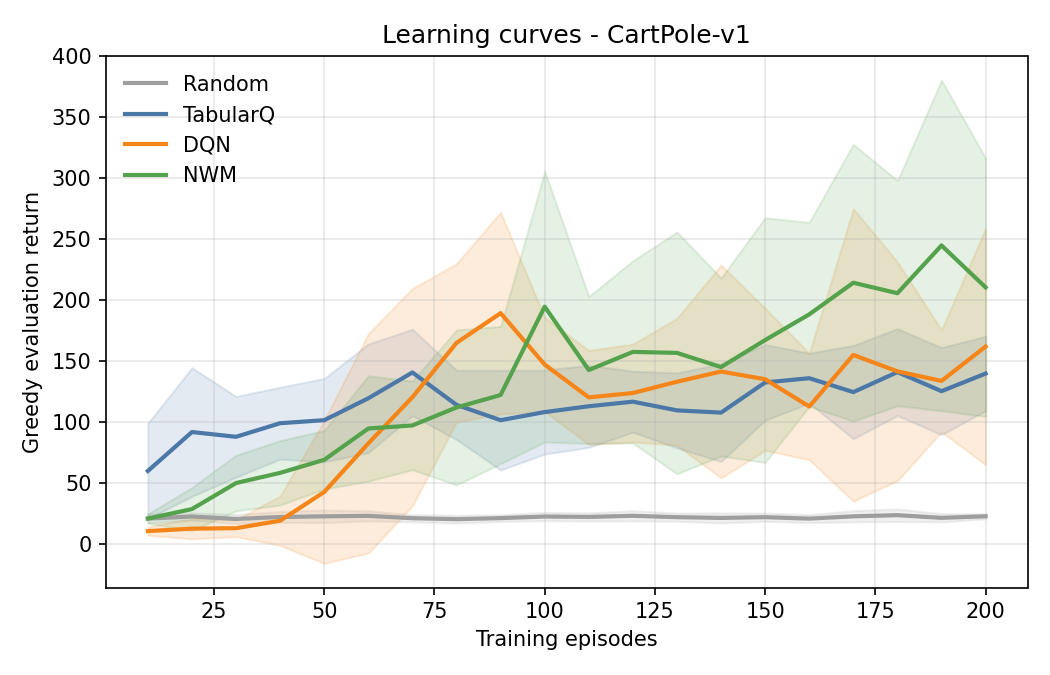
\includegraphics[width=0.32\textwidth]{figures/learning_cartpolev1.png}\hfill
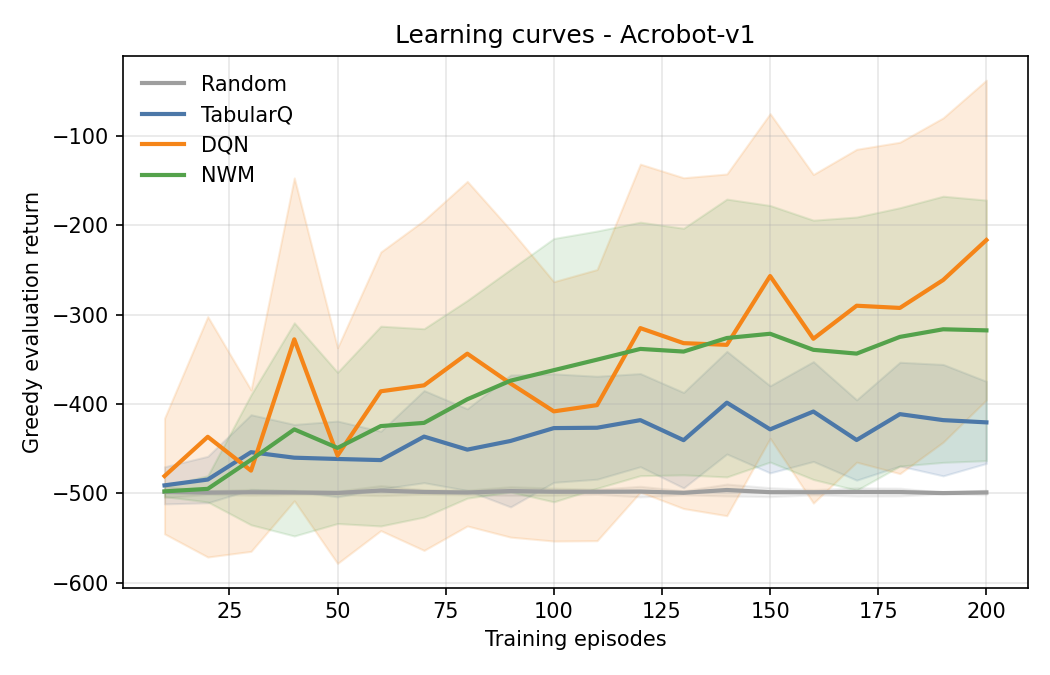
\includegraphics[width=0.32\textwidth]{figures/learning_acrobotv1.png}\hfill
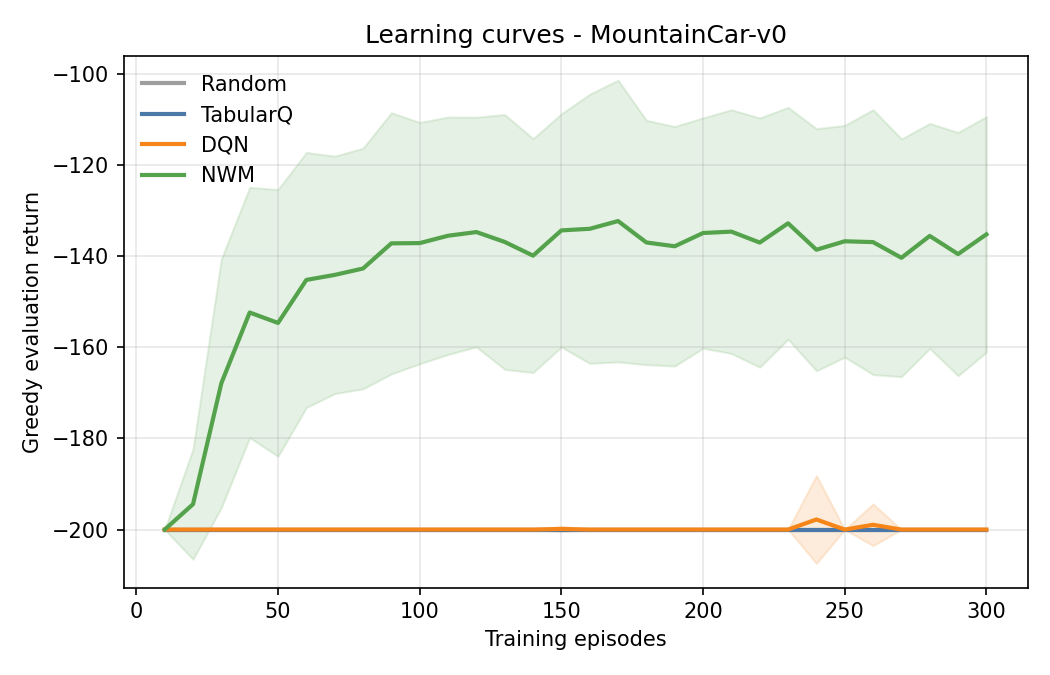
\includegraphics[width=0.32\textwidth]{figures/learning_mountaincarv0.png}
\caption{Greedy-evaluation learning curves (mean over $20$ seeds, shaded
$\pm$ std) for CartPole, Acrobot, and MountainCar.}
\label{fig:curves}
\end{figure}

\begin{figure}[t]
\centering
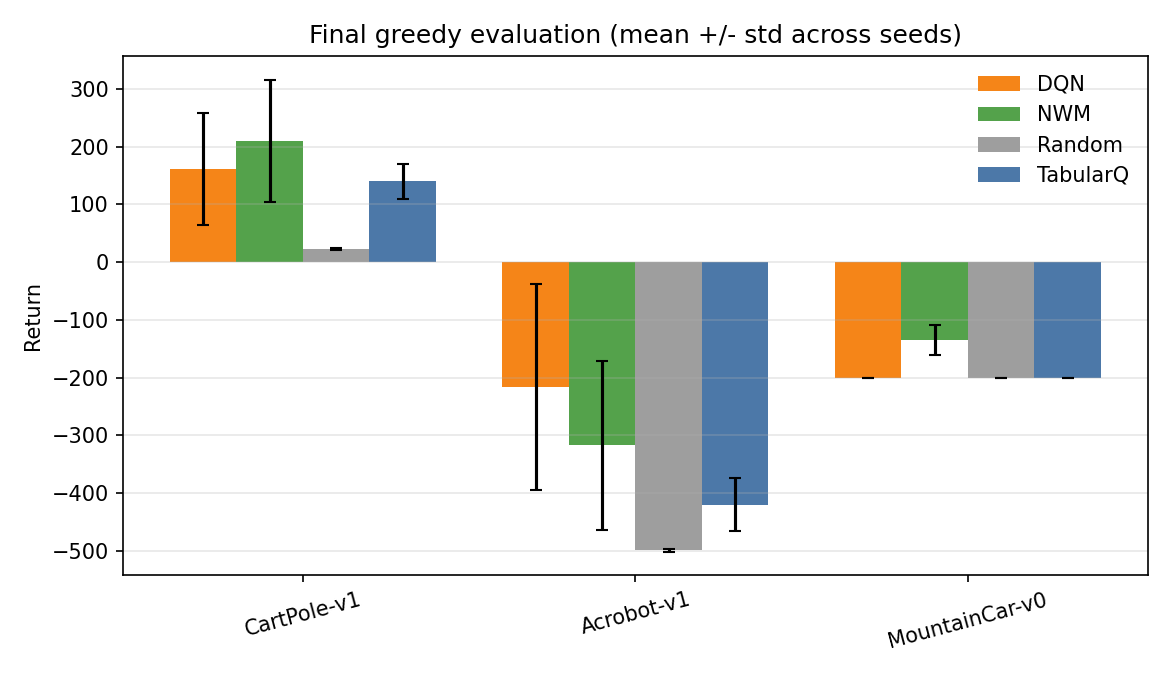
\includegraphics[width=0.7\textwidth]{figures/final_comparison.png}
\caption{Final greedy evaluation per environment and agent (mean $\pm$ std over
$20$ seeds).}
\label{fig:final}
\end{figure}

Because every agent is run on the same seeds, we compare them \emph{paired} per
seed as well as in aggregate; Table~\ref{tab:paired} reports the paired
differences with $95\%$ confidence intervals. We lead with these rather than
with the means of Table~\ref{tab:results}, because two of the three
environments turn out not to support the conclusion their means suggest.

\begin{table}[t]
\centering
\caption{Paired per-seed difference, \NWM{} minus baseline, over the same $20$
seeds. Positive favours \NWM{}. ``Wins'' counts seeds on which \NWM{} scores
higher. $p$ from a Wilcoxon signed-rank test.}
\label{tab:paired}
\small
\begin{tabular}{llccc}
\toprule
Environment & Comparison & $\Delta$ (95\% CI) & Wins & $p$ \\
\midrule
CartPole-v1 & \NWM{} $-$ TabularQ & $+70.7\;[+24.9,+116.4]$ & 13/20 & $0.012$ \\
            & \NWM{} $-$ DQN      & $+48.5\;[-14.3,+111.3]$ & 14/20 & $0.064$ \\
\midrule
Acrobot-v1  & \NWM{} $-$ TabularQ & $+102.9\;[+39.6,+166.3]$ & 13/20 & $0.011$ \\
            & \NWM{} $-$ DQN      & $-101.1\;[-207.3,+5.2]$  & 5/20  & $0.071$ \\
\midrule
MountainCar-v0 & \NWM{} $-$ DQN   & $+64.7\;[+53.1,+76.3]$   & 18/20 & $\mathbf{0.0002}$ \\
\bottomrule
\end{tabular}
\end{table}

\emph{On the sparse-reward task, \NWM{} is decisively the strongest method---and
the failure was exploration, not credit assignment.} MountainCar-v0 gives no
reward until the goal is reached, and \emph{every} baseline---Random, tabular Q,
and DQN alike---finishes at exactly $-200.0\pm0.0$: none reaches the goal once
within the episode budget. \NWM{} reaches $-135.3\pm25.8$, a paired advantage of
$+64.7$ $[+53.1,+76.3]$ on $18$ of $20$ seeds ($p=0.0002$). This is the one
result in the study that is unambiguous, and its cause is identifiable: sticky
exploration builds the momentum needed to crest the hill, the field then forms
around the successful trajectories. Because the only change is the exploratory
action distribution---the scoring and force model are untouched---this isolates
the obstacle. On MountainCar the barrier to a non-bootstrapping method is
generating experience of the goal, not propagating value once it is seen, and a
single task-agnostic exploration change removes it. The mechanism needs no
tuning: the adaptive ramp of Section~\ref{sec:method} sets $p_{\text{rep}}$ from
the agent's own reward history and is what the shared configuration uses.

\emph{On the dense task, \NWM{} has the best mean but the gap to DQN is not
established.} On CartPole-v1 \NWM{} attains $210.6\pm105.9$ against DQN's
$162.1\pm97.0$, and also the better sample efficiency (AUC $135.1$ vs.\
$109.3$). It beats tabular Q-learning significantly ($+70.7$, $p=0.012$). But
the paired advantage over DQN, $+48.5$, has a confidence interval spanning zero
$[-14.3,+111.3]$ and \NWM{} wins on $14$ of $20$ seeds ($p=0.064$). The
defensible claim is that \NWM{} is \emph{competitive with} DQN on this task, not
that it beats it; we previously stated the stronger claim on the strength of a
five-seed run, and it does not survive.

\emph{On the longer-horizon task, DQN is better, though the paired test is
borderline.} On Acrobot-v1 \NWM{} reaches $-317.7\pm145.8$ against DQN's
$-216.6\pm178.9$. The means understate how one-sided the per-seed picture is:
\NWM{} wins only $5$ of $20$ seeds, and the medians diverge much further than
the means ($-272.3$ vs.\ $-87.5$), because DQN's mean is dragged down by a
minority of collapsed runs while its typical run nearly solves the task. Both
methods are strongly bimodal here---a run either learns or sits near the $-500$
floor---which inflates both standard deviations and leaves the paired difference
at $p=0.071$ despite the lopsided win count. We read this as DQN being clearly
better in practice on Acrobot while cautioning that neither the size of the gap
nor its formal significance is well determined at $n{=}20$. \NWM{} does beat
tabular Q-learning here ($+102.9$, $p=0.011$). Longer horizons reward the
temporal credit assignment of bootstrapped value learning that \NWM{}'s episodic
percentile score, even with the propagation of Section~\ref{sec:propagation},
only partly approximates.

\paragraph{Summary.} Of the three environments, one (MountainCar) yields a
strong and well-supported result for \NWM{}, one (CartPole) supports parity with
DQN but not superiority, and one (Acrobot) favours DQN. Two of these three
statements are weaker than the ones this paper made in earlier versions, and the
change came entirely from increasing the seed count rather than from any change
to the method.

\subsection{Ablation: what credit propagation actually buys}
\label{sec:ablation}

Because credit propagation (Section~\ref{sec:propagation}) is the one mechanism
in this release that changes what the field represents, we ablate it directly:
$\beta{=}0.3$ against $\beta{=}0$, on the same $20$ seeds
($\{20,\dots,39\}$, disjoint from both the selection and the reporting seeds),
with every other setting fixed. Because the two configurations share seeds, we
compare them \emph{paired} per seed, which removes the across-seed variance that
dominates these environments. Table~\ref{tab:ablation} reports the result.

\begin{table}[t]
\centering
\caption{Paired ablation of credit propagation over $20$ seeds. $\Delta$ is the
mean per-seed difference ($\beta{=}0.3$ minus $\beta{=}0$); positive favours
propagation. $W$/$L$ counts seeds improved/worsened. Only MountainCar reaches
significance.}
\label{tab:ablation}
\small
\begin{tabular}{lccccc}
\toprule
Environment & $\beta{=}0$ & $\beta{=}0.3$ & $\Delta$ (paired) & $W$/$L$ & Wilcoxon $p$ \\
\midrule
CartPole-v1    & $260.8$  & $269.4$  & $+8.6$  & 10/10 & $0.93$ \\
Acrobot-v1     & $-276.6$ & $-219.2$ & $+57.5$ & 12/8  & $0.37$ \\
MountainCar-v0 & $-159.7$ & $-146.6$ & $+13.1$ & 13/4  & $\mathbf{0.017}$ \\
\bottomrule
\end{tabular}
\end{table}

The honest reading is narrower than we first claimed. On Acrobot---the task
propagation was designed for---the effect is large in the mean ($+57.5$) and in
the right direction, but it is \emph{not} statistically significant
($p=0.37$, and $8$ of $20$ seeds get worse); Acrobot's returns are bimodal, a
run either learns or sits near the $-500$ floor, and the mean is largely a count
of how many runs escaped. On CartPole there is no effect at all
($10/10$ seeds split, $p=0.93$). The only effect that survives a paired test is
on \textbf{MountainCar} ($p=0.017$, $13$ of $20$ seeds improved)---an
environment for which propagation was not designed, and where we had previously
claimed nothing.

We record this because our earlier five-seed measurements told a different and
more flattering story: they showed a clear Acrobot gain bought at a clear
CartPole cost, and we shipped and documented that trade-off. At $n{=}20$ neither
half of it survives---the Acrobot gain is not significant and the CartPole cost
does not exist. The trade-off was an artifact of reading a $\pm60$ standard
error as signal. We keep $\beta{=}0.3$ enabled, since it is neutral-to-positive
on all three tasks and significantly positive on one, but the justification is
not the one we previously gave.

\section{Limitations}
\label{sec:limitations}

\NWM{} has three principal limitations. First, its memory is instance-based, so
query cost grows with the number of centroids and the method targets
low-to-moderate dimensional observation spaces rather than raw pixels.

Second, credit assignment remains weaker than a bootstrapped Bellman backup,
and this is still the residual gap on the longer-horizon Acrobot task. The
propagation of Section~\ref{sec:propagation} narrows it but is \emph{shallow} in
a specific sense: value flows only along transitions the agent has actually
observed and only for a few sweeps, whereas DQN's backups generalize across the
whole state space through the network, including to state-action pairs never
visited consecutively. Propagation on a visited-trajectory graph is closer to
model-free episodic stitching than to dynamic programming, and it inherits the
graph's coverage---sparse regions propagate nothing. Consistent with this, the
ablation of Section~\ref{sec:ablation} cannot establish a significant Acrobot
gain from propagation at $n{=}20$: the mean moves in the right direction, but
$8$ of $20$ seeds still fail to escape the $-500$ floor, which is what a
coverage-limited mechanism would predict. We stress, however, that the
sparse-reward failure mode is genuinely resolved and was never a
credit-assignment problem: on MountainCar the obstacle was exploration, removed
by sticky exploration.

Third, the force model and its constants (thresholds, decays, lock criteria,
the propagation weight $\beta$, and the sticky probability $p_{\text{rep}}$)
are hand-designed. While robust across the tested tasks, they are not learned;
$\beta$ was chosen by a coarse sweep whose intermediate values we would no
longer claim to distinguish, given the noise levels of
Section~\ref{par:power}, and
$p_{\text{rep}}$ trades reactivity for momentum---though it need not be set by
hand, since the adaptive ramp of Section~\ref{sec:method} tunes it from the
agent's own reward history and is what the shared configuration uses.
We view \NWM{} as a transparent, reproducible baseline for non-parametric
control rather than a state-of-the-art method, and a useful component for
hybrid systems.

\paragraph{Negative results.} We also report what did \emph{not} work, since it
sharpens the picture of where the residual Acrobot gap comes from. We
implemented (i) \emph{return-to-go percentile credit}, scoring each step by the
percentile rank of its discounted return-to-go $G_t$ against a rolling history,
with truncated episodes bootstrapping their tail from the running mean per-step
reward; and (ii) an \emph{advantage force model}, replacing the absolute
per-centroid force with each action's score advantage over the \emph{other}
actions observed at the same centroid (an argmax-style local comparison). Both
were ablated on the protocol of Section~\ref{sec:experiments}: (i) was neutral
on MountainCar and clearly worse on Acrobot ($-378$ to $-400$ vs.\ $-247$ for
the shipped configuration over three seeds), because absolute per-step scores
conflate distance-from-goal with action quality, turning the early states of
good episodes repulsive; (ii) was worse still ($-375$ to $-443$), including
when paired with the proven episode-level credit. The lesson is structural:
\NWM{}'s decision rule---the Fear \& Greed thresholds, the safety veto, the
confidence weights---is co-designed around absolute scores with $0.5$ as the
neutral point, and swapping the force formula without redesigning the rule
breaks the system. Closing the long-horizon gap appears to require joint
redesign, not a drop-in bootstrapping patch; neither variant ships in the
released code.

This diagnosis is what made the propagation of Section~\ref{sec:propagation}
work where those attempts failed: it strengthens credit while leaving the score
scale---and therefore the decision rule---invariant. Three further mechanisms
were implemented, measured, and \emph{not} enabled in the shared configuration,
and we report them for the same reason:
\begin{itemize}
  \item \emph{Recency-weighted scores} (\texttt{score\_ema}): replacing all-time
  per-action sums with exponential moving averages, motivated by the
  non-stationarity of percentile scores (a $0.9$ at episode $10$ does not mean
  what a $0.9$ at episode $190$ means). It helps long-horizon Acrobot markedly
  ($-277.6\to-201.6$ at $\alpha{=}0.3$) but costs both CartPole and
  MountainCar, so it ships off.
  \item \emph{Percentile-based exploration collapse}
  (\texttt{relative\_explore}): replacing the CartPole-scaled absolute
  thresholds $450/300$ with percentiles of the agent's own return history. It is
  principled---the constants are meaningless outside CartPole's reward
  scale---but measurably worse on Acrobot ($-369.7$) in the shared
  configuration. It ships off, available for custom setups.
  \item \emph{Stagnation revival} (\texttt{stagnation\_revival}): snapshotting
  the field on new bests and restoring it after a sustained collapse, targeting
  the bimodal across-seed distributions in which individual runs get trapped.
  On the selection seeds it did not improve the benchmark means (CartPole
  $298.2\to273.1$; Acrobot $-233.1\to-265.4$), so despite its intuitive appeal
  it ships off.
\end{itemize}
We consider a mechanism's measured effect, not its plausibility, the criterion
for shipping it. Two caveats apply to this list. First, all three were measured
under the earlier five-seed protocol, so by the argument of
Section~\ref{par:power} the individual figures should be read as indicative
only; what we retain is the decision (none is enabled by default), not the
precise magnitudes. Second, ``did not help'' at that sample size is a statement
about our evidence rather than about the mechanisms, and we would not treat any
of the three as refuted---\texttt{score\_ema} in particular targets a real
defect, the non-stationarity of percentile scores, and deserves a properly
powered re-evaluation.

\section{Conclusion}
\label{sec:conclusion}

We formalized \NWM{}, a potential-field, non-parametric RL framework, and
evaluated it against Random, tabular Q-learning, and DQN on three
classic-control tasks with a reproducible, seed-controlled protocol, using a
single shared configuration and a held-out seed split so that neither
per-task tuning nor a handicapped baseline flatters the method. The study
clarifies the operating regime of instance-based potential-field control and
provides an honest, open baseline: \NWM{} is competitive on dense short-horizon
control, decisively better on the sparse-reward task where exploration rather
than credit assignment is the barrier, and still behind a correctly implemented
DQN on the longest-horizon task.

Credit propagation on the centroid graph (Section~\ref{sec:propagation}) shows
that some of the long-horizon gap is recoverable without abandoning the
non-parametric design, provided the propagation is expressed in the score space
the decision rule already speaks. The natural next steps follow from where it
falls short: propagation over a \emph{learned} similarity structure rather than
only over observed transitions, so that value generalizes into unvisited
regions; learned embeddings for higher-dimensional inputs; and hybrid schemes
that use the repulsive field as an interpretable safety layer around a
parametric policy.

\section*{Reproducibility Statement}
The library, benchmark harness, exact seeds, hyperparameters, and the scripts
that regenerate every table and figure in this paper are released at
\url{https://github.com/CastermustOfficial/NWM}. Running the benchmark and
\texttt{paper/make\_paper\_assets.py} regenerates
\texttt{tables/results\_table.tex} and the figures used above.

\bibliographystyle{plainnat}
\bibliography{references}

\end{document}
